%\pdfoutput=1 % only if pdf/png/jpg images are used
\documentclass{article}
\usepackage{amssymb}
%\usepackage[dvips]{graphicx}
\usepackage{graphicx}
\usepackage{verbatim}
\usepackage{xspace}
\usepackage{hyperref}
\newcommand{\E}{EIGER\xspace}  
\newcommand{\p}{sls\_detector\_put}
\newcommand{\g}{sls\_detector\_get}

\begin{document}

\title{\E - short manual}
\date{\today}
\maketitle
\tableofcontents

\section{Usage}

\subsection{Mandatory setup - Hardware}
An EIGER single module (500~kpixels) needs:
\begin{itemize}
\item A chilled (water+alcohol) at approximately 21~$^{\circ}$C, which needs to dissipate 85~W. For the 9M, a special cooling liquid is required: 2/3 deionized water and 1/3 ESA Type 48.
\item A power supply (12~V, 8~A). For the 9~M, a special cpu is give to remotely switch on and off the detector: see section~\ref{bchip100}. 
\item 2$\times$1~Gb/s Ethernet connectors to control the detector and, optionally, receive data at low rate. A DHCP server that gives IPs to the 1~Gb/s connectors of the detector is needed. Note that flow control has to be enabled on the switch you are using.
\item 2$\times$10~Gb/s transceivers to optionally, receive data at high rate.
\end{itemize}
The equipment scales linearly with the number of modules.
Figure~\ref{fig:1} shows the relationship between the \textbf{Client} (which sits on a beamline control PC), the \textbf{Receiver} (which can run in multiple instances on one or more PCs which receive data from the detector. The receiver(s) does not necessary have to be running on the same PC as the client.) It is important that the receiver is closely connected to the detector (they have to be on the same network). Note that if you implement the 1Gb/s readout only: client, receiver and detector have to be all three in the same network. If you implement the 10Gb/s readout, then client, the 1~GbE of the detector and the receiver have to stay on the 1GbE. But the receiver data receiving device and the 10GbE detector can be on their private network, minimizing the missing packets.  

\begin{figure}[t]
\begin{center}
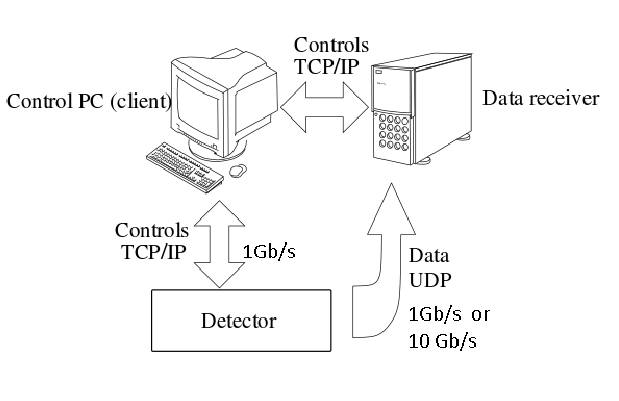
\includegraphics[width=.8\textwidth]{Client2}
\end{center}
\caption{Communications protocol between the Client PC, the receiver PC and the detector.}
\label{fig:1}
\end{figure}

The Client talks to control over 1~Gb Ethernet connection using TCP/IP to the detector and to the receiver. The detector sends data in UDP packets to the receiver. This data sending can be done over 1~Gb/s or 10~Gb/s. 
 
\begin{itemize}
\item \textbf{Switch on the detector only after having started the chiller: the 500k single module and the 1.5M at cSAXS have a hardware temperature sensor, which will power off the boards if the temperature is too high. Note that the detector will be power on again as soon as the temperature has been lowered. The 9M will not boot up without the correct waterflow and temperature has it has an integrated flowmeter.} 
\item \textbf{Switch on the detector only after having connected all the cables and network. EIGER is unable to get IP address after it has been switched on without a proper network set up. In that case switch off and on the detector again.}
\end{itemize}

\subsubsection{9M power supply interface: bchip100}\label{bchip100}
So the bchip100, which is a blackfin cpu, is located on the top side of the 9M and needs to be connected over 1Gb, to the same or a different network as the detector 1~GbE. 
 \begin{verbatim}
telnet bchip100
cd 9m/
\end{verbatim}
The directory contains some executables that are needed to make your detector to work:
 \begin{verbatim}
./on #to switch modules on
./off #to switch modules off
./hvget #gets the current HV value
./waterflow #returns the current waterflow returned by the flowmeter
./temp #returns the water temperature returned by the flowmeter
 \end{verbatim}
A watchdog is running on bchip100 to check for the flow and temperature. If outside of parameters ( flow$<$ 80 dl/min, temperature $\neq$21$\pm$2), the detector will be switched off. 
Here is an explanation of the LED color scheme of the bchip100: 
\begin{itemize}
\item NO LED  Main Power off or Blackfin not ready, yet.
\item RED     Too high temperature or too less water flow
        Detector is shut down and locked.
        Detector will be unlocked (YELLOW) automatically when conditions are good again.
\item YELLOW  Detector is off and unlocked. Ready to be turned on.
\item GREEN   Detector is on
\end{itemize}
You can also Check temperatures and water flow in a browser (from the same subnet where the 9M is: http://bchip100/status.cgi

\subsection{Mandatory setup - Receiver}

The receiver is a process run on a PC closely connected to the detector. Open one receiver for every half module board (remember, a module has two receivers!!!) . Go to {\tt{slsDetectorsPackage/bin/}}, \textbf{slsReceiver} should be started on the machine expected to receive the data from the detector.

\begin{itemize}
\item {\tt{./slsReceiver --rx\_tcpport xxxx}} 
\item {\tt{./slsReceiver --rx\_tcpport yyyy}}
\end{itemize}
where xxxx, yyyy are the tcp port numbers. Use 1955 and 1956 for example. Note that in older version of the software {\tt{--mode 1}} was used only for the ``bottom'' half module. Now, the receiver for the bottom is open without arguments anymore, but still in the configuration file one needs to write {\tt{n:flippeddatax 1}}, where {\tt{n}} indicated the half module number, 1 if it is a module.
\\ Open as many receiver as half module boards. A single module has two half module boards.

From the software version 3.0.1, one can decide weather start a zmq callback from the receiver to the client (for example to visualize data in the slsDetectorGui or another gui). If the zmq steam is not required (cased of the command line for example, one can switch off the streaming with {\tt{./sls\_detector\_put rx\_datastream 0}}, enable it with {\tt{./sls\_detector\_put rx\_datastream 1}}. In the case of inizialising the stream to use the slsDetectorGui, nothing needs to be taken care of by the user. If instead you want to stream the streaming on different channels, the zmq port of the client can be set stealing from the slsDetectorGui stream having {\tt{./sls\_detector\_put n:zmqport 300y}}, where n is each half module independently, matching the receiver stream {\tt{./sls\_detector\_put n:rx\_zmqport 300y}}.
 

There is an example code that can be compiled in {\tt{manual/manual-api/mainReceiver.cpp}} and gives the executable {\tt{./detReceiver}}, use it with two or more receivers to open all receivers in one single terminal: {\tt{./detReceiver startTCPPort numReceivers withCallback}}, where startTCPPort assumes the other ports are consecutively increased.

 


\subsection{Mandatory setup - Client}

\underline{In the case of cSAXS, the detector software is installed on:}\\
\underline{/sls/X12SA/data/x12saop/EigerPackage/slsDetectorsPackage}

The command line interface consists in these main functions:
\begin{description}
\item[sls\_detector\_acquire] to acquire data from the detector
\item[sls\_detector\_put] to set detector parameters
\item[sls\_detector\_get] to retrieve detector parameters
\end{description}

First, your detector should always be configured for each PC that you might want to use for controlling the detector. All the examples given here show the command {\tt{0-}}, which could be omitted for the EIGER system $0$. In the case more EIGER systems are controlled at once, the call of {\tt{1-}},.. becomes compulsory. 

To make sure the shared memory is cleaned, before starting, one should do:  
\begin{verbatim}
sls_detector_get 0-free
\end{verbatim}
To do that:
\begin{verbatim}
sls_detector_put 0-config mydetector.config
\end{verbatim}

In the config file, if client, receiver and detector are using \textbf{1GbE} the following lines are mandatory (see slsDetectorsPackage/examples/eiger\_1Gb.config):
\begin{verbatim}
detsizechan 1024 512 #detector geometry, long side of the module first
hostname beb059+beb058+ #1Gb detector hostname for controls
0:rx_tcpport 1991 #tcpport for the first halfmodule                 
0:rx_udpport 50011 #udp port first quadrant, first halfmodule         
0:rx_udpport2 50012 #udp port second quadrant, first halfmodule       
1:rx_tcpport 1992 #tcpport for the second halfmodule               
1:rx_udpport 50013 #udp port first quadrant, second halfmodule       
1:rx_udpport2 50014 #udp port second quadrant, second halfmodule      
rx_hostname x12sa-vcons #1Gb receiver pc hostname
outdir /sls/X12SA/data/x12saop/Data10/Eiger0.5M
threaded 1
\end{verbatim}

In the config file, if client, receiver and detector commands are on 1Gb, but detector data to receiver are sent using \textbf{10GbE} the following lines are mandatory (see slsDetectorsPackage/examples/eiger\_10Gb.config):
\begin{verbatim}
detsizechan 1024 512 #detector geometry, long side of the module first
hostname beb059+beb058+ #1Gb detector hostname for controls
0:rx_tcpport 1991 #tcpport for the first halfmodule                 
0:rx_udpport 50011 #udp port first quadrant, first halfmodule       
0:rx_udpport2 50012 #udp port second quadrant, first halfmodule       
0:rx_udpip 10.0.30.210 #udp IP of the receiver over 10Gb              
0:detectorip 10.0.30.100  #first half module 10 Gb IP 
1:rx_tcpport 1992 #tcpport for the second halfmodule                  
1:rx_udpport 50013 #udp port first quadrant, second halfmodule     
1:rx_udpport2 50014 #udp port second quadrant, second halfmodule  
1:rx_udpip 10.0.40.210  #udp IP of the receiver over 10Gb, 
                        can be the same or different from 0:rx_udpip                                   
1:detectorip 10.0.40.101 #second half module 10 Gb IP 
rx_hostname x12sa-vcons #1Gb receiver pc hostname
outdir /sls/X12SA/data/x12saop/Data10/Eiger0.5M
threaded 1
\end{verbatim}


In the case you are developing your own receiver, then you need to remove the 1Gb receiver hostname {\tt{rx\_hostname}} and substitute it with the mac address of the device:
\begin{verbatim}
configuremac 0
rx_udpmac xx:xx:...
\end{verbatim}


One can configure all the detector settings in a parameter file {\tt{setup.det}}, which is loaded by doing:
\begin{verbatim}
sls_detector_put 0-parameters setup.det
\end{verbatim}

In the case of \E, the proper bias voltage of the sensor has to be setup, i.e. the {\tt{setup.det}} file needs to contain the line {\tt{vhighvoltage 150}}. Other detector functionality, which are rarely changed can be setup here. 
Other important settings that are configured in the {\tt{setup.det}} file are:
\begin{itemize}
\item {\tt{tengiga 0/1}}, which sets whether the detector is enabled to send data through the 1~or the 10~Gb Ethernet.
\item {\tt{flags parallel/nonparallel}}, which sets whether the detector is set in parallel acquisition and readout or in sequential mode. This changes the readout time of the chip and affects the frame rate capability (faster is {\tt{parallel}}, with higher noise but needed when the frame rate is $>2$~kHz. 
\item {\tt{dr 32/16}} sets the detector in autosumming mode (32 bit counter or not autosumming, 12 bit out of the chip). This is strictly connected to what is required for the readout clock of chip. See next point.
\item {\tt{clkdivider 0/1/2}}. Changes the readout clock: 200, 100, 50~MHz (also referred to as full, half, quarter speed). Note that autosumming mode ({\tt{dr 32}} only works at {clkdivider 2}=quarter speed). By selecting Refer to readout timing specifications in~section\ref{timing} for how to set the detector. 
\item {\tt{flags continuous/storeinram}}. Allows to take frame continuously or storing them on memory. Normally {\tt{continuous}} should be used. Enabling the  {\tt{stroreinram}} mode allows you to obtain the maximum frame rate, but at the expenses to have to receive the data all at the end of the acquisition. Refer to readout timing specifications in section~\ref{timing} for how to set the detector.
\end{itemize}

One should notice that, by default, by choosing the option {\tt{dr 32}}, then the software automatically sets the detector to  {\tt{clkdivider 2}}. By choosing the option {\tt{dr 16}}, the software automatically sets the detector to  {\tt{clkdivider 1}}. One needs to choose {\tt{clkdivider 0}} after setting the {\tt{dr 16}} option to have the fastest frame rate. 
We would recommend expert users (beamline people) to write their parameters file for the users. 

\section{API versioning}
The eigerDetectorServer running on the boards has a versioning API scheme that will make it crash if used with a wrong firmware.
You can also check your versioning by hand with the code:
\begin{verbatim}
 sls_detector_get softwareversion
\end{verbatim}
gets the server (slsDetectorSoftware) version (answer is something like: {\tt{softwareversion 111920160722}}.
 \begin{verbatim}
sls_detector_get thisversion 
\end{verbatim}
returns the client version. The answer can be {\tt{thisversion 111220160718}}.
\begin{verbatim}
/sls_detector_get detectorversion
\end{verbatim}
returns the firmware version . The answer can be {\tt{detectorversion 11}}.
Killing and starting the server on the boards allows you to check the firmware version you have and also if your board is a top/bottom/master/slave.

\section{Setting up the threshold}
\begin{verbatim}
sls_detector_put 0-trimen N xxxx yyyy zzzz
sls_detector_put 0-settings standard #[veryhighgain/highgain/lowgain/verylowgain] also possible
sls_detector_put 0-threshold energy_in_eV
\end{verbatim}
The first line requires to specify how many ({\tt{N}}) and at which energies in eV {\{tt{xxxx}}, {\tt{yyyy}}, {\tt{zzzz}} and so on) trimmed files were generated (to allow for an interpolation). This line should normally be included into the {\tt{mydetector.config}} file and should be set for you by one of the detector group.
NORMALLY, in this new calibration scheme, only {\tt{settings standard}} will be provided to you, unless specific cases to be discussed.
The threshold at 6000 eV , for example would be set as:{\tt{sls\_detector\_put 0-threshold 6000}}.

We have added a special command, {\tt{thresholdnotb}}, which allows to scan the threshold energy without reloading the trimbits at every stage. One can either keep the trimbits at a specific value (es.32 if the range of energies to scan is large) or use the trimbits from a specific energy (like a central energy).
\begin{verbatim}
sls_detector_put 0-thresholdnotb energy_in_eV
\end{verbatim}

\section{Standard acquisition}

After you setup the setting and the threshold, you need to specify the exposure time, the number of real time frames and eventually how many real time frames should be acquired:
\begin{verbatim}
sls_detector_put 0-exptime 1[time_is_s]
sls_detector_put 0-frames 10
sls_detector_put 0-period 0[time_is_s]
\end{verbatim}
In this acquisition 10 consecutive 1~s frames will be acquired. Note that {\tt{period}} defines the sum of the acquisition time and the desired dead time before the next frame. If {\tt{period}} is set to 0, then the next frame will start as soon as the detector is ready to take another acquisition. \\

For \E, at the moment 5 settings are possible: {\tt{standard}}, {\tt{lowgain}}, {\tt{verylowgain}}, {\tt{veryhighgain}} and {\tt{highgain}}. According to the setting chosen, one can reach different requirements (low noise or high rate). Refer to the settings requirements for your detector.\\ 
Notice that the option {\tt{settings standard/highgain/lowgain/veryhighgain/verylowgain}} actually loads the trimbit files so it is time consuming. Only setting the {\tt{threshold}} does not load trimbit files.  

The threshold is expressed in (eV) as the proper threshold setting, i.e. normally is set to 50\% of the beam energy.  

\underline{At cSAXS, the {\tt{settingsdir}} and {\tt{caldir}} are in}\\\underline{/sls/X12SA/data/x12saop/EigerPackage/calibrations/}\\ 

You need to setup where the files will be written to
\begin{verbatim}
sls_detector_put 0-outdir /scratch
sls_detector_put 0-fname run
sls_detector_put 0-index 0
\end{verbatim}
this way your files will all be named /scratch/run\_dj\_i.raw where $j$ is relative to each specific half module, $i$ in the {\tt{index}} starts from 0 when starting the detector the first time and is automatically incremented. The next acquisition {\tt{index}} will be 1. One can reset the  {\tt{index}} to what wished.

To acquire simply type:
\begin{verbatim}
sls_detector_acquire 0-
\end{verbatim}
Note that acquiring is blocking.
You can poll the status of the detector with:
\begin{verbatim}
sls_detector_get status
\end{verbatim}
If the detector is still acquiring, the answer will return {\tt{running}}. If the detector has finished and ready for the next acquisition, then it will return {\tt{idle}}.
You can also ask for the status of the receiver, to know when it has returned and finished getting the data with:
\begin{verbatim}
sls_detector_get receiver
\end{verbatim}

There is a more complex way of performing an acquisition, that is useful for debugging and in case one wants a non blocking behavior: 
\begin{itemize}
\item {\tt{sls\_detector\_put 0-receiver start}} 
\item {\tt{sls\_detector\_put 0-status start}} 
\end{itemize}

You can poll the detector status using:
\begin{verbatim}
sls_detector_get 0-status 
\end{verbatim}
When the detector is {\tt{idle}}, then you need to stop the receiver doing:
\begin{itemize}
\item {\tt{sls\_detector\_put 0-receiver stop}} 
\end{itemize}
You can then reset to zero the number of frames caught, if you desire:
\begin{itemize}
\item {\tt{sls\_detector\_put 0-resetframescaught 0}} 
\end{itemize}

The detector will not accept other commands while acquiring. If an acquisition wishes to be properly aborted, then:
\begin{itemize}
\item {\tt{sls\_detector\_put 0-status stop}} 
\end{itemize}
this same command can be used after a non proper abortion of the acquisition to reset to normal status the detector.

\section{Readout timing- maximum frame rate}\label{timing}
IMPORTANT: to have faster readout and smaller dead time, one can configure {\tt{clkdivider}}, i.e. the speed at which the data are read, i.e. 200/100/50~MHz for {\tt{clkdivider 0/1/2}} and the dead time between frames through {\tt{flags parallel}}, i.e. acquire and read at the same time or acquire and then read out.
The configuration of this timing variables allows to achieve different frame rates. NOTE THAT IN EIGER, WHATEVER YOU DO, THE FRAME RATE LIMITATIONS COME FROM THE NETWORK BOTTLENECK AS THE HARDWARE GOES FASTER THAN THE DATA OUT.

In the case of REAL CONTINUOUS readout, i.e. continuous acquire and readout from the boards (independent on how the chip is set), the continuous frame rates are listed in table~\ref{tcont}:
\begin{table} 
\begin{tabular}{|c|c|c|c|}
\hline
GbE & dynamic range & continuos maximum frame rate(Hz) & minimum period ($\mu$s)\\
\hline
1 & 16 &  \textbf{256} & 3901\\ 
\hline 
1 &  32 &  \textbf{128} & 7820\\
\hline 
10 & 16 & \textbf{2560} & 391\\  
\hline 
10 & 32 & \textbf{1280}& 782\\  
\hline 
10 & 8 & \textbf{5120} & 196\\
\hline
10 & 4 & \textbf{10240} & 98\\
\hline
\end{tabular}
\caption{Frame rate limits for the CONTINUOS streaming out of images.} 
\label{tcont}\end{table}
Note that in the {\tt{continuous}} flag mode, some buffering is still done on the memories, so a higher frame rate than the proper real continuous one can be achieved. Still, this extra buffering is possible till the memories are not saturated. 
The number of images that can be stored on memories are listed in table~\ref{timgs}:
\begin{table}
\begin{tabular}{|c|c|}
\hline
dynamic range & images\\
\hline
4 & 30000\\
\hline
8 & 15000\\
\hline
16 & 7600\\
\hline
\end{tabular}
\caption{Amount of images that can be stored on board. As while we store them, we start to send them out, the effective number of images could be larger than this, but it will depend on the network setup (how fats you stream out images).}
\label{timgs}
\end{table}

The maximum frame rate achievable with 10~GbE, {\tt{dr 16}}, {\tt{flags continuous}}, {\tt{flags parallel}},{\tt{clkdivider 0}}, \textbf{6.1~kHz}. This is currently limited by the connection between the Front End Board and the Backend board. We expect the 32 bit mode limit to be \textbf{2~kHz} ({\tt{clkdivider 2}}).
 In dynamic range {\tt{dr 8}} the frame rate is \textbf{11~kHz} and for{\tt{dr 4}} is \textbf{22~kHz}. For 4 and 8 bit mode the frame rate are directly limited by the speed of the detector chip and not by the readout boards.    

In table~\ref{tframes} is a list of all the readout times in the different configurations:
\begin{tiny}
\begin{table}
\begin{flushleft}
\begin{tabular}{|c|c|c|c|c|c|c|c|}
\hline
\tiny{dr} & \tiny{clkdivider} & \tiny{flags} & \tiny{readout t($\mu$s)} & \tiny{max frame rate (kHz)} & \tiny{max exptime ($\mu$s)} & \tiny{min period ($\mu$s)} & \tiny{max imgs (nominal/our network)}\\
\hline
4 & 0 & parallel & 3.4 & 22 &  40 & 44 & 30k/50k\\
\hline
4 & 0 & nonparallel & 44 & 21 &  3 & 49 & 30k/50k\\
\hline
4 & 1 & parallel & 6 & 10.5 &  85 & 92 & 30k/100k\\
\hline
4 & 1 & nonparallel & 88.7 & 10.5 & 3 & 93 & 30k/100k\\
\hline
4 & 2 & parallel & 11.2 & 5.4 &  185 & 197 & infinite\\
\hline
4 & 2 & nonparallel & 176.5 & 5.4 &  3 & 180 & infinite\\
\hline
\hline
8 & 0 & parallel & 3.4 & 11.1 &  85 & 89 & 15k/24k\\
\hline
8 & 0 & nonparallel & 85.7 & 11.1 & 3 & 91 & 15k/24k\\
\hline
8 & 1 & parallel & 6.1 & 5.7 &  174 & 181 & 15k/52k\\
\hline
8 & 1 & nonparallel & 170.5 & 5.7 &  3 & 175 & 15k/52k\\
\hline
8 & 2 & parallel & 11.2 &  2.9 &  330 & 342 & infinite\\
\hline
8 & 2 & nonparallel & 340.3 &  2.9 &  3 & 344 & infinite\\
\hline
\hline
16 & 0 & parallel & 3.4 & 6 & 164 & 168 & 8k/12k\\
\hline
16 & 0 & nonparallel &  126 & 3.4& 164 & 295 & 8k/23k\\
\hline
16 & 1 & parallel &  6.1 & 2.9&  339 & 346 & 8k/28k\\
\hline
16 & 1 & nonparallel & 255 & 1.7&  339 & 592 & infinite\\
\hline
16 & 2 & parallel &  11 & 1.5& 66 & 78 & infinite \\
\hline
16 & 2 & nonparallel & 504 & 0.85 & 7 & 512 & infinite\\
\hline
\hline
32 & 2 & parallel &  11 & 2&  & &\\
\hline
32 & 2 & nonparallel & 504 & $<2$&  & &\\
\hline
\end{tabular}
\caption{Readout settings. The {\tiny{min exptime}} possible is 5$-$10~$\mu$s. This is due to the time to pass the pixel enable signal in the whole chip.}
\label{tframes}
\end{flushleft}
\end{table}
\end{tiny}
\textbf{As if you run too fast, the detector could become noisier, it is important to match the detector settings to your frame rate. This can be done having more parameters files and load the one suitable with your experiment.} We experienced that {\tt{highgain}} settings could not be used at 6~kHz.
\textbf{We recommend to use the detector in 32 bit mode with {\tt{clkdivider 2}}, {\tt{flags parallel}}. We recommend to use the detector in 16 bit mode with {\tt{clkdivider 1}}, {\tt{flags parallel}}}. In general, choose first the desired dead time: this will tell you if you want to run in parallel or non parallel mode. Then, choose the maximum frame rate you want to aim, not exceeding what you aim for not to increase the noise.


\section{External triggering options}
The detector can be setup such to receive external triggers. Connect a LEMO signal to the TRIGGER IN connector in the Power Distribution Board. The logic 0 for the board is passed by low level 0$-$0.7~V, the logic 1 is passed to the board with a signal between 1.2$-$5~V. Eiger is 50~$\Omega$ terminated. By default the positive polarity is used (negative should not be passed to the board).  
\begin{verbatim}
sls_detector_put 0-timing [auto/trigger/burst_trigger/gating]
sls_detector_put 0-frames x
sls_detector_put 0-cycles y
sls_detector_acquire 0-
\end{verbatim}
No timeout is expected between the start of the acquisition and the arrival of the first trigger. 

Here are the implemented options so far:
\begin{itemize}
\item {\tt{auto}} is the software controlled acquisition, where {\tt{exptime}} and {\tt{period}} have to be set.
\item {\tt{trigger}} 1 frame taken for 1 trigger. You {\tt{frames}} needs to be  1 always, {\tt{cycles}} can be changed and defines how many triggers are considered. In the GUI this is called trigger exposure series. 
\item {\tt{burst\_trigger}} gets only 1 trigger, but allows to take many frames. With {\tt{frames}} one can change the number of frames. {\tt{cycles}} needs to be 1. In the gui it is called trigger readout.
\item{\tt{gating}} allows to get a frame only when the trigger pulse is gating. Note that in this case the exp time and period only depend on the gating signal. {\tt{cycles}} allows to select how many gates to consider. 
\end{itemize}

Hardware-wise, the ENABLE OUT signal outputs when the chips are really acquiring. This means that the single subframes will be output in 32 bit mode. The TRIGGER OUT outputs the sum-up-signal at the moment (which is useless). This will be changed in the future to output the envelop of the enable signal. 

We are planning to change some functionality, i.e. unify the {\tt{trigger}} and {\tt{burst}} trigger modes and make both {\tt{frames}} and {\tt{cycles}} configurable at the same time.

\section{Autosumming and rate corrections}

In the case of autosumming mode, i.e, {\tt{dr 32}}, the acquisition time ({\tt{exptime}} is broken in as many subframes as they fit into the acquisition time minus all the subframes readout times. By default the {\tt{subexptime}} is set to 2.621440~ms. This implies that 12 bit counter of \E will saturate when the rate is above or equal to 1.57~MHz/pixel. The minimum value is of order of 10~ns (although as explained values smaller than 500~$\mu$s do not make sense). The maximum value is 5.2~s.

The subframe length can be changed by the user by doing: 
\begin{verbatim}
sls_detector_put 0-subexptime [time_in_s] 
\end{verbatim}

One needs to realize that the readout time, for each subframe is 10.5~$\mu$s if the detector is in parallel mode. 500~$\mu$s if the detector is in non parallel mode. Note that in {\tt{dr 32}}, as the single frame readout from the chip is 500~$\mu$s, no {\tt{subexptime}}$<$500~$\mu$s can be set in {\tt{parallel}} mode. To have smaller {\tt{subexptime}}, you need the {\tt{nonparallel}} mode, although this will have a larger deadtime than the acquisition time.\\

Rate corrections are possible online (and the came procedure can be used offline) by creating a look-up table between the theoretically incident counter value $c_i$ and the detected counter value $c_d$. 
In the EIGER on board server, this look-up table is generated assuming that the detected rate $n_d$ can be modeled as a function of the incident rate $n_i$ according to the paralyzable counter model:
\begin{equation}
n_d= n_i \cdot exp(-n_i \cdot \tau),
\label{rate}
\end{equation}
where $\tau$ represents an effective parameter for the dead time and the loss in efficiency. The look-up table is necessary as we are interested to obtain $c_i(c_d)$ and equation~\ref{rate} is not invertible. One needs to notice that the paralizable counter model to create a look-up tables applies only if photons arrive with a continuous pattern (like at the SLS). If photons are structured in fewer but intenser bunches, deviations may arise. This is the case for some operation modes at the ESRF. For those cases we are studying how to correct, probably from a simulated correction tables if an analytical curve cannot be found.  
\textbf{In the new calibration scheme, $\tau$ is given as a function of the energy. It is loaded from the trimbit files and interpolation between two trimbit files are performed.} One needs to make sure the appropriate $\tau$ value is written in the trimbit files, then need to load the appropriate {\tt{settings}} and {\tt{vthreshold}} before.

Online rate corrections can be activated for {\tt{dr=32}}. They are particularly useful in the autosumming mode as  every single subframe is corrected before summing it. To correct for rate, the subframe duration has to be known to the correction algorithm. Rate corrections for {\tt{dr=16}} will be activated as well in the next firmware release.     
To activate the rate corrections, one should do:\\
\begin{verbatim}
sls_detector_put 0-ratecorr [tauval_in_ns]
\end{verbatim}
To deactivate:
\begin{verbatim}
sls_detector_put 0-ratecorr 0
\end{verbatim}

 Now to activate the rate corrections with the value written in the trimbit file or interpolated from there, once would do: 
\begin{verbatim}
sls_detector_put 0-ratecorr -1
\end{verbatim}

Every time either the rate corrections are activated, $\tau$ is changed or the subframe length is changed, then a new correction table is evaluated. Note that computing the correction table is time consuming. 

\section{Dependent parameters and limits}
Here is a list of dependent parameters:
\begin{enumerate}
\item \textbf{dr} changes \textbf{clkdivider}: \textbf{dr} 16 $\to$  \textbf{clkdivider} 1. You can change it to (0, 1, 2); the frame rate changes accordingly to table~\ref{tframes}. Setting the \textbf{dr} to 32 changes \textbf{clkdivider} to 2. Only way  \textbf{dr} 32 can work. 
\end{enumerate}

Here is a list of "ignored'' parameters, meaning that if the parameters are not what the detector expects, it will ignore them, but there is no guarantee that you get what you think you are asking: 
\begin{enumerate}
\item \textbf{period}. Assuming that you set the correct \textbf{exptime} according to the table~\ref{tframes}, the \textbf{period} to be used by the detector has to be $>=$ \textbf{exptime}+readout time (table~\ref{tframes}). Otherwise the detector will take data at the minimum possible period, which is \textbf{exptime}+readout times. \textbf{period} is not changed by the detector after the acquisition. 
\end{enumerate}

Here is a list of limits that should be checked:
\begin{enumerate}
\item 
If \textbf{dr} is 32 and \textbf{clkdivider} is not 2, whatever the detector gets out is wrong (the boards cannot properly keep up) 
\item If the variable \textbf{frames} is greater than what the memory can store (table~\ref{timgs}) and the frame rate exceed the continuos streaming (table~\ref{tcont}), limits on the maximum number of images need to be implemented if the period is lower than the one listed in table~\ref{tcont}. Check table~\ref{tframes} to see the different cases.
\item Running at a speed that does not support the frame rate you are asking: see table~\ref{tframes} to check if the frame rate (\textbf{period}) you are asking is compatible with the \textbf{clkdivider} you are asking.
\item Running at a redout time that does not support the frame rate you are asking. Check table~\ref{tframes} to check if the frame rate (\textbf{period}) you are asking is compatible with the \textbf{flags} you are asking.
\item The minimum allowed value for \textbf{exptime} should be 10~$\mu$s. 
\item By default the {\textbf{subexptime}} is set to 2.621440~ms. Values smaller than 500~$\mu$s do not make sense. The maximum value is 5.2~s. This limits should be checked.
\end{enumerate}


\section{1Gb/s, 10Gb/s links}
\subsection{Checking the 1Gb/s, 10Gb/s physical links}\label{led}
LEDs on the backpanel board at the back of each half module signal:
\begin{itemize}
\item  the 1Gb/s physical link is signaled by the most external LED (should be green) 
\item the 10Gb/s physical link is signaled by the second most external LED next to the 1Gb/s one (should be green) 
\end{itemize}

\subsection{Delays in sending for 1Gb/s, 10Gb/s, 10Gb flow control, receiver fifo}

Extremely advanced options allow to:
\begin{itemize}
\item Activate the flow control for 10~Gb/s~E (by default the 1~Gb/s~E is always active and cannot be switched off:
\begin{verbatim}
./sls_detector_put flowcontrol_10g 1
\end{verbatim}
\item  Delay the transmission of the left port. This delay option is useful in the case of many simultaneous receivers running, such that it reduces the throughput to the receivers all at the same time. To be used board by board (i.e {\tt{X:, Y:,etc..}} with different units:
\begin{verbatim}
./sls_detector_put X:txndelay_left xxxx 
\end{verbatim}
\item  Transmission delay of the right port, same as above. The value here should be different from the left port to spread the transmission even more 
\begin{verbatim}
./sls_detector_put X:txndelay_right yyyy
\end{verbatim}
As example:
\begin{verbatim}
for X in \$(seq 0 4); do ./sls_detector_put \$X:txndelay_left \$((X*100000)); done
 \end{verbatim}
\begin{verbatim}
./sls_detector_put \$X:txndelay_right \$((X*100000)); X=\$((X+1)); done
\end{verbatim}

\item Set transmission delay of the entire frame. This is required as you want to finish sending the first frame to all receivers before starting sending the second frame to the receivers with shorter delay time.  This value has to be greater than the maximum of the transmission delays of each port.      
\begin{verbatim}
./sls_detector_put txndelay_frame zzzz
\end{verbatim}
In the example before, it would be: {\tt{zzzz}}=4*100000+ 100000

\item Readjust the size of the fifo of the receiver between listening and writing (useful when writing is limited)
\begin{verbatim}
./sls_detector_put rx_fifodepth xxxx
\end{verbatim}
 {\tt{xxxx}} is 100 images by default.
\item Deactivate a half module (for ROI or debugging). Note that the MASTER module SHOULD NOT be deactivated:
\begin{verbatim}
./sls_detector_put X:activate 0 
\end{verbatim}
where $X$ is the half module you want to deactivate.
The receiver at this point will return fake data (overflow) for this module. If you wish to eliminate the receiver overall for this module, then you need to run a configuration file where this module has been removed.
To activate back a module, do:
\begin{verbatim}
./sls_detector_put X:activate 1
\end{verbatim}

\end{itemize}
\subsection{Setting up 10Gb correctly: experience so far}\label{10g}

For configuring well the 10Gb card not to loose packets, 
\begin{itemize}
\item MTU must be set up to 9000 (jumbo frames) on all the involved sides: detector, switch, server NIC
\item you should set up static MAC address tables with separated VLANs
\end{itemize}
As root, also do:
\begin{verbatim}
 ethtool -G xth1 rx 4096, ethtool -C xth1 rx-usecs 100 
\end{verbatim}
where {\tt{xth1}} can be replaced with the correct 10Gb device. To minimise loosing packets, priorities are set better as root user, so have the receiver as root.
To try to bypass being root, we trued something like this:
\begin{verbatim}
/etc/security/limits.conf  username – rtprio 99
\end{verbatim}
but somehow it did  not fully worked  so we kept the trick of being root.

Very important is to activate the flow control in 10Gb (in 1Gb it is on by default and not configurable)
\begin{verbatim}
./sls_detector_put flowcontrol_10g 1
\end{verbatim}
Set the transmission delays as explained in the manual.

\section{Offline processing and monitoring}

\subsection{Data out of the detector: UDP packets}

The current UDP header format is described in figure~\ref{UDPheader}.
\begin{figure}[t]
\begin{center}
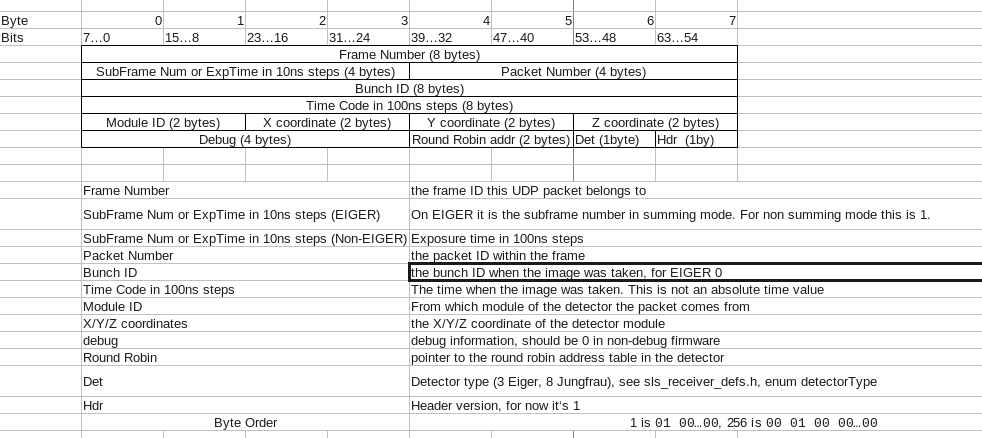
\includegraphics[width=1.2\textwidth]{EIGERUDPHeader}
\end{center}
\caption{UDP header out of EIGER}
\label{UDPheader}
\end{figure}
 
\subsection{Data out of the slsReceiver}


For a module, the geometry of the ports are as in table~\ref{tports}: 
\begin{table}
\begin{tabular}{|c|c|}
\hline
{\tt{0:rx\_udpport 50011}} &  {\tt{0:rx\_udpport2 50012}}\\  
\hline
{\tt{1:rx\_udpport 50013}} &  {\tt{1:rx\_udpport2 50014}}\\  
\hline
\end{tabular}
\caption{UDP port geometry for a single module, 4 UDP ports.}
\label{tports}
\end{table}
white the option {\tt{n:flippeddatax 1}}, which flips in vertical the content of the module. By convection, we usually use {\tt{1:flippeddatax 1}}, but one could flip the top instead.


\subsection{``raw'' files}
If you use the option of writing raw files, you will have a raw file for each UDP port (meaning most likely 2 chips), 4 files per module. In addition to the raw files, you will get also a ``master'' file, containing in ascii some detector general parameters and the explanation of how to interpret the data from the raw files.
   
The master file is named: {\tt{filename\_master\_0.raw}} and for version ``3.0'' of the slsDetectorSoftware looks like:
 
\begin{verbatim}
Version            : 1.0
Dynamic Range      : 16
Ten Giga           : 1
Image Size         : 262144 bytes
x                  : 512 pixels
y                  : 256 pixels
Total Frames       : 1
Exptime (ns)       : 1000000000
SubExptime (ns)    : 2621440
Period (ns)        : 1000000000
Timestamp          : Thu Aug 17 10:55:19 2017


#Frame Header
Frame Number       : 8 bytes
SubFrame Number    : 4 bytes
Packet Number      : 4 bytes
Bunch ID           : 8 bytes
Timestamp          : 8 bytes
Module Id          : 2 bytes
X Coordinate       : 2 bytes
Y Coordinate       : 2 bytes
Z Coordinate       : 2 bytes
Debug              : 4 bytes
Round Robin Number : 2 bytes
Detector Type      : 1 byte
Header Version     : 1 byte
\end{verbatim}

Note that if one wants to  reconstruct the real time the detector was acquiring in 32 bit (autosumming mode), one would have to multiply the SubExptime (ns) for the SubFrame Number. 

\subsection{Offline image reconstruction}
The offline image reconstruction is in {\tt{slsDetectorsPackage/slsImageReconstruction}}.

The detector writes a raw file per receiver. An offline image reconstruction executable has been written to collate the possible files together and produce cbf files. The executable uses the CBFlib-0.9.5 library (downloaded from the web as it download some architecture dependent packages at installation).\\
\underline{At cSAXS, the CBFlib-0.9.5 has been compiled -such that the required packages are}\\\underline{ downloaded in /sls/X12SA/data/x12saop/EigerPackage/CBFlib-0.9.5.}\\ 

To use it for a single module:
\begin{verbatim}
cbfMaker [filename with dir]
\end{verbatim}
eg.
{\tt{cbfMaker /scratch/run\_63\_d1\_f000000000000\_3.raw}}\\

To use it for a 1.5 multi modules:
\begin{verbatim}
cbfMaker [filename] [pixels x] [pixels y] ([singlemodulelongside_x] [start det])
\end{verbatim}
eg.
{\tt cbfMaker /scratch/run\_63\_d0\_f000000000000\_3.raw  3072 512 1 0}.\\
The {\tt{[singlemodulelongside\_x]}} and {\tt{[start det]}} param are optional. Defaults are ``1'', the detector long side is on the x coordinate and start to reconstruct from module 0. 
The executables: 
\begin{verbatim}
bcfMaker1.5M [file_name_with_dir]
bcfMaker9M [file_name_with_dir]
\end{verbatim}
contain the hardcoded geometry for the 1.5M (3 modules horizontal on the long side) and for the 9M at cSAXS: 6(short side)$\times$3 (long side) modules.\\ 
Missing packets in a frame and border pixels ($\times 2$ and $\times 4$ are given with value $-1$ at the present time.

It is important to know, that the pixels at the edge between 2 chips count more as double size. We can virtually introduced 1 virtual pixel per double larger pixel, so to have an even number of counts everywhere. Virtual pixels (not filled ) between module gaps are also inserted.

 \begin{verbatim}
   GapPixelsBetweenChips_x = 2;
   GapPixelsBetweenChips_y = 2;
   GapPixelsBetweenModules_x = 8;
   GapPixelsBetweenModules_y = 36;
 \end{verbatim}

\subsection{Read temperatures/HV from boards}

With an updated kernel on the linux boards (ask to the SLS detector group for specifications), it is possible to monitor the temperature on the boards: 
\begin{verbatim}
temp_fpga   #gets the temperature of the fpga
temp_fpgaext   #gets the temperature close to the fpga
temp_10ge   #gets the temperature close to the 10GE
temp_dcdc   #gets the temperature close to the dc dc converter
temp_sodl   #gets the temperature close to the left so-dimm memory
temp_sodr   #gets the temperature close to the right so-dimm memory
temp_fpgafl   #gets the temperature of the left front end board fpga
temp_fpgafr   #gets the temperature of the right front end board fpga

\end{verbatim}

You need to use the command specifying from which board you desire the temperature readings, for example:
\begin{verbatim}
./sls_detector_get 0:temp_fpga
./sls_detector_get 1:temp_fpga
\end{verbatim}
In 500k--2M pixel systems there is a hardware temperature safety switch, which will cut power to the BEBs when reaching a too high temperature. For the 9M system, there is a temperature sensor read by the bchip100 PCU which will shutdown the detector when above a certain temperature.
 
The HV can also be set and read through the software:
\begin{verbatim}
./sls_detector_put vhighvoltage 150
./sls_detector_get vhighvoltage 
\end{verbatim}
Note that the get {\tt{vhighvoltage}} would return the measured HV from the master module only. If getting the vhighvoltage for individual halfmodules, only the master will have a value different from -999.

\appendix

\section{Kill the server, copy a new server, start the server}\label{server}
All the below operations are form a terminal and assume you login to the boards.\\
Kill current server:
\begin{verbatim}
ssh root@bebxxx #password is root
killall eigerDetectorServer # kill server and stopserver
\end{verbatim}
Copy a new version of the server (if necessary, otherwise skip it):
\begin{verbatim}
cd executables
scp user@pc:/path/eigerDetectorServerNewVersion .
chmod 777 eigerDetectorServerNewVersion
mv eigerDetectorServerNewVersion eigerDetectorServer
sync
\end{verbatim}
Start the server again:
\begin{verbatim}
./eigerDetectorServer &
\end{verbatim}


\section{Loading firmware bitfiles}

A \textbf{bcp} executable (which needs \textbf{tftp} installed on the PC, is needed. 
\begin{enumerate}
\item Manual way: you need to press something on the detector. To program bitfiles (firmware files), do a hard reset with a pin/thin stuff in the holes at the very back of the module. They are between the top 7 LED and the bottom 1 and opposite for the other side. Push hard till all LEDs are alternating green and red.
\item Software way (possible only if you have the correct programs copied on your board. If not, as the sls detector group). 
\begin{verbatim}
ssh root@bebxxx
cd executables
./boot_recovery 
 \end{verbatim} 
\end{enumerate}
In both case, after booting, only the central one should be on green and red alternating. 

From a terminal, do:
\begin{verbatim}
nc -p 3000 -u bebxxx 3000 
\end{verbatim} 
where {\tt{xxx}} is the board number. It is enough top monitor with {\tt{nc}} only one board. Pres enter twice (till you see a prompt with the board hostname printed) and keep this terminal to monitor. It takes a bit of time to load the bitfiles, but the terminal tells you.\\
From another terminal you do:
\begin{verbatim}
./bcp feb_left.bit bebxxx:/febl
sleep 300; #or till the screen over netcat has told you Successful
./bcp feb_right.bit bebxxx:/febr
sleep 300; #or till the screen over netcat has told you Successful
./bcp download.bit bebxxx:/fw0
sleep 300; #or till the screen over netcat has told you Successful
\end{verbatim}
If you need to program a new kernel (only needed when told to do so):
\begin{verbatim}
 ./bcp kernel_local bebxxx:/kernel
sleep 300; #or till the screen over netcat has told you Successful
\end{verbatim}
do the same for the other boards. You can program in parallel many boards, but you cannot load two bitfiles on the same board till loading and copying one process has finished. So load all left febs together, then proceed to the right febs, then the bebs. Power off completely everything. Power it on.

\section{Pulsing the detector}
There are two ways to pulse the detector: 
\begin{itemize}
\item \textbf{Pulse digitally:} when you are interested to the output readout and do not care about the analog response from the pixels:
 \begin{verbatim}
sls_detector_put vthreshold 4000
sls_detector_put vtr 4000
sls_detector_put pulsechip N #to pulse N
sls_detector_put pulsechip -1 #to get out of testing mode 
\end{verbatim}
Note that the answer will be $2 \cdot \textrm{{\tt{N}}} +2$ in this case.

\item  \textbf{Pulse analogically:} You want to really check the analogical part of the detector, not just the readout.

 \begin{verbatim}
sls_detector_put vcall 3600
sls_detector_put vthreshold 1700
sls_detector_put vrf 3100
for i in $(seq 0 7) ; 
do px=$((-255+i)); 
sls_detector_put  pulse 0 $px 0;
for j in $(seq 0 255) ; do
sls_detector_put pulsenmove N 0 1;
done;
done;
sls_detector_p resmat 0
sls_detector_acquire
\end{verbatim}
You read {\tt{N}} in every pixel if you are setup correctly. 
\end{itemize}
 
\section{Load a noise pattern with shape}
For debug purposes, we have created a noise pattern with a shape. If you reconstruct correctly your image, you should be able to read ".EIGER'' in the same direction for both the top and bottom in normal human readable orientation.
To load the special noise file look at {\tt{settingsdir/eiger/standard/eigernoise.sn0xx}} in the package. 
\begin{verbatim}
sls_detector_put trimbits ../settingsdir/eiger/standard/eigernoise
\end{verbatim}

\section{Running the (9M at cSAXS. For now)}
\begin{itemize}
\item login as {\tt{x12saop@xbl-daq-27}}
\item {\tt{setup\_eiger}} \#loads environmental variables and brings you to the right directory to execute commands
\item slsReceiverScript3 1991 36 \# from one shell.. opens 36 receivers
\item p config ../../eiger\_9m\_10gb\_xbl-daq-27\_withbottom.config
\end{itemize}

\section{Troubleshooting}
\subsection{Cannot successfully finish an acquisition}
\subsubsection{only master module return from acquisition}
When no packets are received AND detector states in 'running status'. Widest list of causes. 
Query the status of each half module till the maximum number {\tt{N}},  {\tt{for i in \$(seq\ 0\ N); do sls\_detector\_get \$i:status; done}}, to check if there are half modules that are still running.

If only the master modules return but ALL the other half modules do not: 
\begin{itemize}
\item FEB LED 1 and or 3 become red while trying to acquire an image: reconnect or change the DDR2 memories. Technically it is a FIFO problem to communicate the data to the rest of the chain. 
\item It can be that the master cable is not connected, check.
\item It can be that the synchronization cable is not connected or the termination board at the synchronization does not work. Check.
\end{itemize}

\subsubsection{a few modules do not return from acquisition}
If only a few modules are still running but the others return, it is a real problem with a backend board or a synchronization bug.
If you can, ssh into the board, kill and start the eigerDetectorServer again (see Section~\ref{server} for how to do this). Keep the terminal with the output from the  eigerDetectorServer and repeat the acquisition. 
\begin{itemize}
\item Check if the acquisition returned from the server or not. In case seek help from the SLSDetectorGroup.
\item In the server you read something along the lines of "cannot read top right address". It is communication between the front and backend board. Or FEB FPGA is not programmed. Try to program again FPGA, and make sure you program FPGA bit files 70x, if you have 70x FPGAs, or 30x, if you have 30x FPGAs. If still fails, tell the SLSDetectorGroup as it could be a hardware permanent failure.
\end{itemize}

\subsection{No packets (or very little) are received} 
In both cases running \textbf{wireshark} set to receive UDP packets on the ethernet interface of the receiver (filter the UDPport$>=$xxxx, where xxxx is written in the configuration file) can help you understanding if NO packets are seen or some packets are seen. You have to set the buffer size of the receiving device in wireshark to 100Mbyte minimum. If no packets are received, check that your receiving interface and detector UDPIPs are correct (if in 10Gb). Most of the time in this case it is a basic configuration problem.
If some packets are received, but not all, then it is an optimization problem:
 \begin{itemize}
\item For receiving data over 1Gb, the switch must have FLOW CONTROL enabled 
\item If using 10GbE, check that the 10Gb link is active on the backpanel board. Then refer to Section~\ref{10g} to see how to configure the 10Gb ports on the receiving machine correctly. 
\end{itemize}

\subsection{The module seems dead, no lights on BEBs, no IP addresses}
\begin{itemize}
\item Check the 2 fuses on the power distribution board. If one of the fuses is in shortcuircuit, then exchange it. Nominal values are 7 A and 5 A. Old modules with 5 A and 3 A could trip.
\item The module is not properly cooled and the temperature safety switch has killed the power to the backend boards. 
\end{itemize}

\subsection{The module seems powered but no IP addresses}
If the 1G LED (see Section~\ref{led}) on the backpanel board is not green:
\begin{itemize}
\item Check that the 1Gb cable is plugged in.
\item Check that there is a DCHP server assigning IP addresses to the board.
\item The IP address is assigned only at booting up of the boards. Try to reboot in case the board booted before it could have an IP address. 
\item Check that you did not run out of IP addresses 
\end{itemize}
 Check that the board is not in recovery mode (i.e. the central LED on the back is stable green). In this case reboot the board with the soft reset or power cycle it.

If the 1Gb LED on the backpanel board is green (see Section~\ref{led}):
\begin{itemize}
\item Check that the IP address has been refreshed on the PC you are trying to communicate to the detector from. Run on the PC as root the following command to update the DNS cache: \textbf{nscd -i hosts} 
\end{itemize}

\subsection{Receiver cannot open socket}
It is connected to the TCPport which the receiver uses:
\begin{itemize}
\item The port is already in use by the same receiver already opened somewhere or by another process: check with \textbf{ps -uxc} your processes
\item In rare cases, it might be that the TCP port crashes. To find out which process uses the TCPPOrt do: \textbf{netstat -nlp | grep xxxx}, where xxxx is the tcpport number. To display open ports and established TCP connections, enter: \textbf{netstat -vatn}. Kill the process.
%%%#To display only open UDP ports try the following command: netstat -vaun
 \end{itemize}

\subsection{Client has \textbf{shmget error}}
Note that occasionally if there is a shared memory of a different size (from an older software version), it will return also a line like this:
\begin{verbatim}
*** shmget error (server) ***-1
\end{verbatim}
This needs to be cleaned with {\tt{ipcs -m}} and then {\tt{ipcrm -M xxx}}, where xxx are the keys with nattch 0. Alternative in the main slsDetectorFolder there is a script that can be used as {\tt{sh cleansharedmemory.sh}}. Note that you need to run the script with the account of the client user, as the shared memory belongs to the client. It is good procedure to implement an automatic cleanup of the shared memory if the client user changes often.   

\subsection{Measure the HV}
For every system but not the 9M: 
\begin{itemize}
\item Software-wise measure it (now the software returns the measured value), with {\tt{sls\_detector\_get vhighvoltage}}. The returned value is the HV (for proper Eiger setting is approximately 150~V) if it is correctly set. If two master modules are presents (multi systems), the average is returned (still to be tested). If one asks for the individual $n$ half module bias voltage through {\tt{sls\_detector\_get n:vhighvoltage}}, if the $n$ module is a master, the actual voltage will be returned. If it is a slave, -999 will be returned. 
\item Hardware-wise measure value of HV on C14 on the power distribution board. Check also that the small HV connector cable is really connected. 
 \end{itemize}

\subsection{The image now has a vertical line}
Check if the vertical line has a length of 256 pixels and a width of 8 columns. In this case it is a dataline beeing bad. It can be either a wirebond problem or a frontend board problem. try to read the FEB temperature (see Section~\ref{}) and report the problem to the SLSDetector group. Most likely it will be a long term fix by checking the hardware.

\subsection{The image now has more vertical lines}

If you see strange lines in vertical occurring at period patterns, it is a memory problem. The pattern is 4 columns periodic in 16 bit mode, 8 columns periodic in 8 bit mode and 2 columns periodic in 32 bit mode. Try to switch on and off (sometimes it is a strange initialization problem).

\subsection{ssh to the boards takes long}
Depending on your network setup,  to speed up the ssh to the boards from a pc with internal dhcp server running: \textbf{iptables -t nat -A POSTROUTING -o eth1 -j MASQUERADE; echo "1" > /proc/sys/net/ipv4/ip\_forward}, where eth1 has to be the 1Gb network device on the pc

\subsection{Check firmware version installed on BEB}
Follow some steps described in Section~\label{server}. 
\begin{verbatim}
ssh root@bebxxx #password is root
killall eigerDetectorServer # kill server and stopserver
cd executables/
./eigerDetectorServer&
\end{verbatim}
Scroll up in the terminal till you find {\tt{Firmware Version: xx}}

\subsection{Check if half-module is a master, a slave, a top or a bottom}
Follow some steps described in Section~\label{server}.
\begin{verbatim}
ssh root@bebxxx #password is root
killall eigerDetectorServer # kill server and stopserver
cd executables/
./eigerDetectorServer&
\end{verbatim}
Scroll up in the terminal till you find:\\
*************** TOP/BOTTOM ***************\\
*************** MASTER/SLAVE ***************\\
*************** NORMAL/SPECIAL ***************\\




\section{Client checks - command line}

Guide on returned strings:
\begin{enumerate}
\item \begin{verbatim}
sls_detector_get free
\end{verbatim}
Returns a list of shared memories cleaned (variable number depending on detector):
\begin{verbatim}
Shared memory 273612805 deleted
Shared memory 276922374 deleted
Shared memory 270270468 deleted
free freed
\end{verbatim}
Note that occasionally if there is a shared memory of a different size (from an older software version), it will return also a line like this:
\begin{verbatim}
*** shmget error (server) ***-1
\end{verbatim}
This needs to be cleaned with {\tt{ipcs -m}} and then {\tt{ipcrm -M xxx}}, where xxx are the keys with nattch 0. 
\item \begin{verbatim}sls_detector_get settings
settings standard
\end{verbatim} 
{\tt{standard}} is only if correct. {\tt{undefined}} or anything else is wrong. 

\item \begin{verbatim}
sls_detector_get threshold
threshold xxxx
\end{verbatim}
Returns a string (xxxx) that can be interpreted as the threshold in eV. If it fails to set it, returns the last threshold it was set (which the detector still has). If settings are not defined or different trimbits are chosen, it will return "undefined".

\item \begin{verbatim}
sls_detector_get fname
fname string
\end{verbatim}

\item \begin{verbatim}
sls_detector_get exptime
exptime number
\end{verbatim}
where {\tt{number}} is a string to be interpreted as a float in (s). 

\item \begin{verbatim}
sls_detector_get period
period number
\end{verbatim}
where {\tt{nuymber}} is a string to be interpreted as a float in (s). 

\item \begin{verbatim}
sls_detector_get frames
frames number 
\end{verbatim}
where {\tt{number}} is a string to be interpreted as an integer.

\item \begin{verbatim}
sls_detector_get cycles
cycles number 
\end{verbatim}
where {\tt{number}} is a string to be interpreted as an integer.

\item \begin{verbatim}
sls_detector_get status
status string 
\end{verbatim}
where {\tt{string}} can be {\tt{idle}} or {\tt{running}}.

\item \begin{verbatim}
sls_detector_get index
status number
\end{verbatim}
where {\tt{number}} is a string to be interpreted as an integer.

\item \begin{verbatim}
sls_detector_get dr
dr number
\end{verbatim}
where {\tt{number}} is a string that should be interpreted as an integer (4/8/16/32).

\item \begin{verbatim}
sls_detector_get clkdivider
clkdivider number
\end{verbatim}
where {\tt{number}} is a string that should be interpreted as an integer (0/1/2/3).

\item \begin{verbatim}
sls_detector_get flags
flags string1 string2 
\end{verbatim}
where {\tt{string1}} is a string should be always {\tt{continous}} and {\tt{string2}} can be either {\tt{nonparallel}} or {\tt{parallel}}.

\item \begin{verbatim}
sls_detector_get timing 
timing string
\end{verbatim}
where {\tt{string}} is a string which can be {\tt{auto/trigger/burst\_trigger/gating}}.

\item \begin{verbatim}
sls_detector_get enablefwrite
enablefwrite number
\end{verbatim}
where {\tt{number}} is a string which should be interpreted as an integer "0" or "1".

\item \begin{verbatim}
sls_detector_get framescaught
framescaught number
\end{verbatim}
where {\tt{number}} is a string which should be interpreted as an integer of the complete frames got by the receiver.

\item \begin{verbatim}
sls_detector_get frameindex
frameindex number
\end{verbatim}
where {\tt{number}} is a string which should be interpreted as an integer of the last frame number read from firmware. It comes from the receiver, though and reset after every acquisition series.

\item \begin{verbatim}
sls_detector_get subexptime
subexptime number
\end{verbatim}
where {\tt{number}} is a string that should be interpreted as a float in s. The default value is 0.002621440. 

\item \begin{verbatim}
sls_detector_get ratecorr
ratecorr number
\end{verbatim}
where {\tt{number}} is a string that should be interpreted as a float in s.  0.000000 means correction off. Values above zero are the value of $\tau$ in ns.

\item \begin{verbatim}
sls_detector_get vhighvoltage
vhighvoltage number
\end{verbatim}
where {\tt{number}} is a string that should be interpreted as an int and for proper Eiger setting is approximately 150~V if it is correctly set. If two master modules are presents (multi systems), the average is returned (still to be tested). If one asks for the individual $n$ half module bias voltage through {\tt{sls\_detector\_get n:vhighvoltage}}, if the $n$ module is a master, the actual voltage will be returned. If it is a slave, -999 will be returned. 
  
\item \begin{verbatim}
sls_detector_get busy
busy number
\end{verbatim}
where  {\tt{number}} is a string that should be interpreted as an int for 0/1 meaning no/yes. This command tells if the sharedmemory has in memory that an acquisition has been started or not. It should allows to use the non blocking acquire, regardless of any delay to the detector getting into 'running' mode. 


\end{enumerate}



\end{document}

